\documentclass[10pt]{exam}
\usepackage[phy]{template-for-exam}
\usepackage{tikz}
\usetikzlibrary{shadings,decorations.pathmorphing,arrows.meta,patterns}

\title{The Godfather of All Mechanics Problems}
\author{Rohrbach}
\date{\today}

\begin{document}
\maketitle

\noindent
You can complete this problem by test day for 5 bonus points!  Even if you don't get it totally correct, you will get partial bonus for attempting.  {\bf Note that you will need to use physics from both the Momentum unit and the Energy unit to solve!}

\vspace{2em}

A force of 20~N is applied to a 2-kg block for 0.28~s.  It then travels at a constant velocity along a frictionless surface before coming to a frictionless ramp that is 3~m high and at a 20-degree angle.  At the bottom of the ramp, it encounters a friction force of $-2$~N.  How far from the bottom of the ramp (the value $d$ on the diagram) will the block slide until coming to a stop? (\emph{Hint:} Use the diagram below to label the values you might have.  You will need to break the problem into smaller parts.)

\vspace{3em}

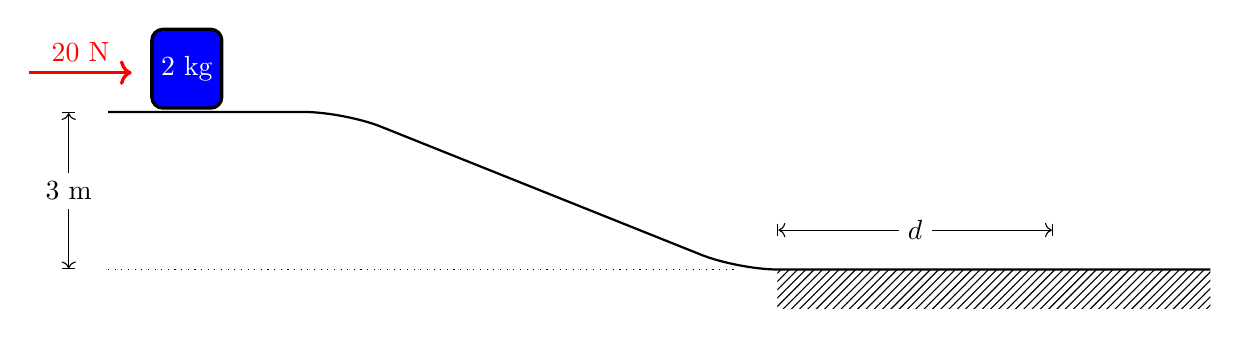
\begin{tikzpicture}
  \draw[thick, rounded corners=0.5cm] 
    (0,2) -- (3,2) -- (8,0) -- (14,0); 
  \fill[pattern=north east lines] 
    (8.5,0) rectangle (14,-.5);
  %\draw[fill=blue, rounded corners, very thick] 
  %  (0.1,2) rectangle ++(0.5,0.5);
  \node[
      white, 
      fill=blue, 
      rounded corners,
      draw=black, 
      very thick,
      minimum height=1cm
    ] 
    at (1,2.55) {2 kg};
  \draw[->,very thick, red] 
    (-1,2.5) -- ++(1.3,0) 
    node[midway,above] {20 N};

  \draw[|<->|] (8.5,0.5) -- (12,0.5)
    node[midway,fill=white] {$d$};

  \draw[|<->|] (-0.5,0) -- (-0.5,2)
    node[midway,fill=white] {3 m};

  \draw[dotted] (0,0) -- (8,0);
  
\end{tikzpicture}


\end{document}